\documentclass{article}

\usepackage[english]{babel}
\usepackage[utf8]{inputenc}
\usepackage{amsmath}
\usepackage{amssymb}
\usepackage{graphicx}
\usepackage{geometry}
\newtheorem{theorem}{Theorem}
\newtheorem{definition}{Definition}

\title{A Time-Efficient Pok\'emon Competitive Team-Building Algorithm}
\author{Hugo Reijm, 4272692}
%\institute{TU Delft}
\date{\today}
\selectlanguage{english}

\begin{document}
\maketitle
\newpage
\tableofcontents

\newpage
\section{Introduction}
Welcome to the world of Pok\'emon! The Pok\'emon franchise is one that has existed since 1996, starting with the release of the Pok\'emon Red and Pok\'emon Green video games in Japan. Since then, it has become one of the world's most successful "children's entertainment properties" in the world (POKEMON ABOUT US). The Pok\'emon  company specializes in the making of trading cards along side the independent made, but related, video games. This report will focus on the latter.\\\\
One of the reasons for the astounding success the Pok\'emon video games have had, is the incredible amount of variety and complexity present within the games' mechanics. So much potential for variation is present, that it has become difficult for competitive players to decide how to play the game. Therefore, the author developed a computer algorithm to mathematically analyze almost any situation a competitive player finds himself/herself in, and give advice in how to proceed. This algorithm has been named the Scored-Based Pok\'emon Analyzer Algorithm (or SBPA).\\\\
This paper will give an in-depth look at the theory behind SBPA and its workings. However, before the algorithm can be fully understand, one must first understand the Pok\'emon games and more importantly, the mechanics behind competitive Pok\'emon play.

\section{An In-depth Look at Pok\'emon Mechanics}
The Pok\'emon video games are set in a world a little different from reality. This world is filled with creatures called Pok\'emon, short for "Pocket Monster" (REFERENCE). What does a Pok\'emon look like? Almost anything. Just like there are many varying animal species in the real world, so there are many different species of Pok\'emon in the Pok\'emon world. In the case of Pok\'emon, there are currently 721 different species of Pok\'emon, and more are revealed each year. What makes things even more complicated is that several Pok\'emon have multiple forms that they can take on in and out of battle. For the comprehensiveness, the author has for the most part ignored these forms in this report; however he has taken these into account in SBPA.\\\\
For simplicity, the following Pok\'emon will be used as an example from now on:
\begin{center}
	
\includegraphics[width=0.5\textwidth]{fluffy.png}
\end{center}
This is a Pok\'emon nicknamed "Fluffy". He's about the size of a small dog.\\\\
In the Pok\'emon world, People and Pok\'emon live together in harmony. Some people, called trainers, catch and train Pok\'emon like Fluffy in order to battle other trainers and their Pok\'emon. This concept is what the Pok\'emon video games center around: the player becoming stronger by catching and battling other Pok\'emon.\\\\
Over the years, players from all over the world have assembled in places such as Tokyo, Boston, and elsewhere to battle each other in this way. They have strategized and trained their Pok\'emon to peak performance in order to become the best. This is called competitive Pok\'emon battling. This competition has its climax during the world championships, held in a different city every year. How does one of these competitive matches look like?

\subsection{A Typical Pok\'emon Battle}
A typical Pok\'emon battle is fought between 2 players with their collection of 6 Pok\'emon, called a team. Each player may only use one team during a battle, and one team may only have a maximum of 6 Pok\'emon. Also, Pok\'emon battles are divided into certain classifications based on tiers.
\begin{definition}\label{tierdef}
	Not all Pok\'emon are made equal; they are ranked according to their power and potential into sets called \textbf{Tiers}. Two Pok\'emon trainers must clearly agree on which tiers are allowed to be used before engaging in battle. This is done in order to establish not only fairness in battle, but also a diversity in match styles.
\end{definition} 
The SBPA algorithm focuses on 7 different tiers in order to give the user a significant amount of choice. The 8 different tiers are:
\begin{itemize}
	\item \textbf{Anything Goes}, abbreviated AG, which includes all 721 Pok\'emon species, a total of 817 if including Pok\'emon forms
	\item \textbf{Ubers}, which also includes all 721 Pok\'emon species. However, it excludes a certain form of a certain Pok\'emon species, resulting in a total of 816 if including Pok\'emon forms
	\item \textbf{Battle Spot Singles}, abbreviated here as BS, which is the official tier in the Pok\'emon games and includes 690 Pok\'emon species, a total of 753 if including Pok\'emon forms
	\item \textbf{Over Used}, abbreviated OU, which includes 701 Pok\'emon species, a total of 760 if including Pok\'emon forms
	\item \textbf{Under Used}, abbreviated UU, which includes 656 Pok\'emon species, a total of 687 if including Pok\'emon forms
	\item \textbf{Rarely Used}, abbreviated RU, which includes 584 Pok\'emon species, a total of 602 if including Pok\'emon forms
	\item \textbf{Never Used}, abbreviated NU, which includes 527 Pok\'emon species, a total of 539 if including Pok\'emon forms
\end{itemize}
Below is a graph that visualizes the amount of Pok\'emon species and forms allowed in a tier:
\begin{center}
	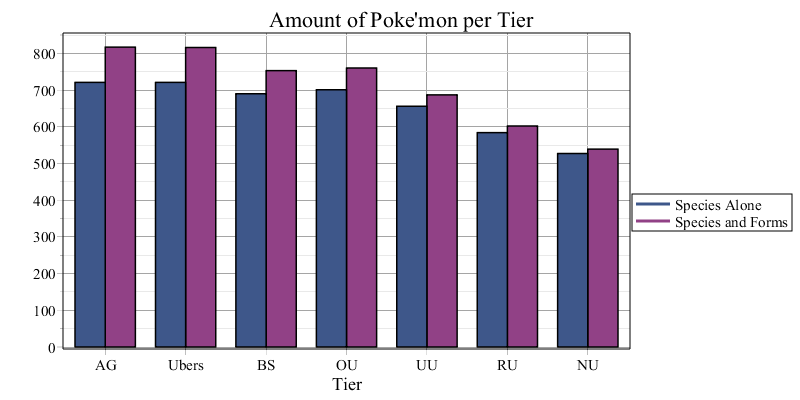
\includegraphics[width=\textwidth]{TierAmount.png}\label{TierAmountGraph}
\end{center}
Furthermore, typically a battle enacts a Species Clause, which limits the player to using only 6 different Pok\'emon species. That being the case, a quick calculation reveals how many groups of 6 different Pok\'emon one can have:
\begin{equation*}
	\left({721 \above 0pt 6}\right)=1.91082439565304\text{ x }10^{14}
\end{equation*}
Roughly 200 trillion different groups of 6 different Pok\'emon exist. Note that this is not the total amount of teams that exist, because individual Pok\'emon from a Pok\'emon species can be widely differing amongst each other. In other words, the amount of actual teams that can be constructs is much larger than the result above. This is the reason why constructing the SBPA algorithm is more complex than just brute-force calculating which team would be best in a certain situation: the runtime to compute this would be far too impractical for such an approach.\\\\
Back to understanding how a typical Pok\'emon battle procedes, the players start by viewing a basic overview of the opponent's team. In this overview, nothing is revealed about the opponents team except which Pok\'emon it contains. Based on this overview, each player privately decides which Pok\'emon to send into battle. Once both players have made their selection, the battle begins.\\\\
A Pok\'emon battle is a turn-based system. Each turn begins with both players privately selecting their preferred actions for that turn. Once both players have decided what they will do for that turn, the results of the players' decisions is played out and a new turn begins. This cycle is repeated until a player has no more usable Pok\'emon to battle with, usually resulting from the player's Pok\'emon being "knocked out" by the opponent's Pok\'emon. When this happens, the player with no more usable Pok\'emon loses the match. In the rare case that both players lose their last Pok\'emon, the victor is decided by who hit last.\\\\
This is a basic oversight of a competitive Pok\'emon battle. Many variations in battle style exist, but all can be boiled down to this system.\\\\
The quality of a Pok\'emon team could therefore be described as follows. The human element in this case is removed from the definition for simplicity's sake.
\begin{definition}
	A Pok\'emon team has quality $\alpha$ when out of the $N$ Pok\'emon battles, the team win $m(\alpha)$ of them, whereby $N$, $m(\alpha)\in\mathbb{N}\cup\{0\}$ and $m(\alpha)\le N$.
\end{definition}
Therefore, for a team to have a high quality, the designer must think of all the factors involved and optimize them. This report will analyze these factors in a bottom-up fashion, relying on the philosophy that one can not fully understand the whole without understanding all the parts. Therefore, the next few sections describe the mechanics of individual Pok\'emon, because one can not fully understand a team without understanding all the intricacies of a single Pok\'emon.

\subsection{Individual Pok\'emon Mechanics}
Pok\'emon, even at an abstract level, are complex objects with many varying characteristics. As per previous, observe Fluffy. He may look simple, but a further analysis reveals the following:
\begin{center}
	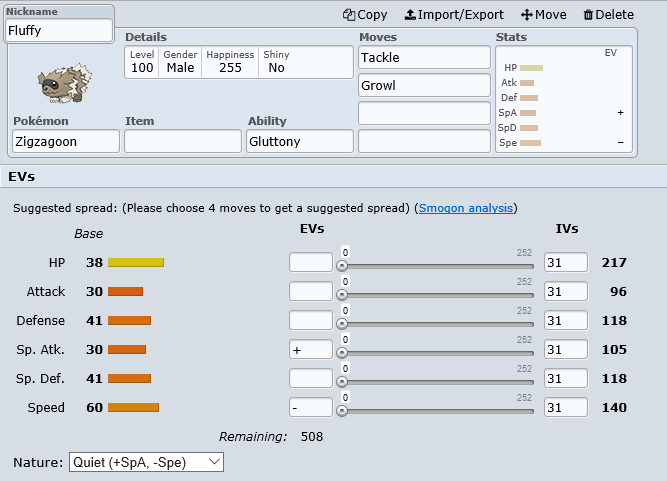
\includegraphics[width=0.9\textwidth]{fluffyfile.png}
\end{center}
This is Fluffy expressed in numbers and figures; a rather large set of mathematical data. What makes Fluffy even more complicated is that many of the factors present here can be different from individual Pok\'emon to individual Pok\'emon. In other words, two individuals from the same species can be vastly different from each other, again strengthening the argument that too many unique Pok\'emon teams exist for brute-force calculations to be a viable option.\\\\
Due to time constraints in the developmental phase, the SBPA algorithm does not take into account many of the factors present here. Therefore, SBPA is an approximation algorithm and merely gives advice; it can not calculate ever single situation to result in a perfect optimum. However, SBPA can still give viable advice by using two important factors found in every Pok\'emon: Base Statistics and Types.

\subsubsection{Base Statistics}
Taking another look at Fluffy and his file, we can see the following section:
\begin{center}
	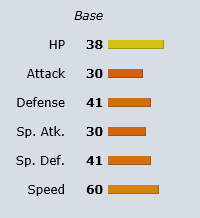
\includegraphics[width=0.4\textwidth]{fluffystats.png}
\end{center}
These are Fluffy's Base Statistics. Base Statistics, also know as "Base Stats", are a set of 6 integers that determine how well a Pok\'emon can fill a certain role in a team. For example, if a Pok\'emon team requires a new member that is incredibly fast, then the trainer will have to search for a Pok\'emon with a very high Speed Stat. \\\\
The following definitions shed light on what each Base Stat stands for:
\begin{definition}
	The \textbf{HP} Base Stat stands for the Health Points that a Pok\'emon has. Very basically, Health Points determines how large of an attack the Pok\'emon of interest can survive.
\end{definition}
\begin{definition}
	The \textbf{Attack} Base Stat stands for the physical power a Pok\'emon possess. If a Pok\'emon were to use a physically attacking move, such as throwing a punch, then the power of that move would be determined in part by this Base Stat. 
\end{definition}
\begin{definition}
	The \textbf{Defense} Base Stat stands for how well a Pok\'emon can defend itself from physical moves. 
\end{definition}
\begin{definition}
	The \textbf{Sp.Atk.} Base Stat (an abbreviation for "Special Attack") stands for the Special power a Pok\'emon possess. The word "Special" refers to any move that doesn't include direct physical contact between the attacking and defending Pok\'emon. Examples for such moves are "Thunderbolt", "Shadow Ball", and "Telekinesis".
\end{definition}
\begin{definition}
	The \textbf{Sp.Def.} Base Stat (an abbreviation for "Special Defense") stands for how well a Pok\'emon can defend itself from Special moves. 
\end{definition}
\begin{definition}
	The \textbf{Speed} Base Stat stands for fast a Pok\'emon is. In a battle, the Speed Base Stat determines which Pok\'emon moves first in a turn.
\end{definition}
A trainer that is building a Pok\'emon team must keep into account how the Base Stats of each team member interact with each other. Perhaps the trainer wants to make a team that is more aggressive than most teams. That would entail that he/she needs to put more focus on the overall Attack, Special Attack, and Speed of his/her team. Perhaps he/she wishes to make a slower, defensive team. Then the overall HP, Defense, and Special Defense of the team are of more importance.\\\\
For simplicity's sake, assume that Base Stats are species-dependent characteristics; that is to say: every individual of a Pok\'emon species has the same Base Stats. Technically, Base Stats can change from individual to individual due to modifiers, but analyzing these would be too complicated and time-consuming. The SBPA algorithm also makes this assumption, therefore resulting in the algorithm not looking at every possible individual of every possible Pok\'emon species, but merely looking a species as a whole.

\subsubsection{Typing}
Another species-dependent characteristic is Typing. Every species can have up to two types, which classify what that Pok\'emon species is. For example, Fluffy is an individual of Pok\'emon species 263 (commonly known as "Zigzagoon"). All individuals of species 263 have only one type: the "Normal" type.\\\\
There are 18 types in total: Bug, Dark, Dragon, Electric, Fairy, Fighting, Fire, Flying, Ghost, Grass, Ground, Ice, Normal, Poison, Psychic, Rock, Steel, and Water. These types interact with each other in a complex game similar to Rock-Paper-Scissors; the situation is more complicated, however, because of Weaknesses, Resistances, and Immunities. The basic definitions are given below:
\begin{definition}
	A type's \textbf{Weaknesses} are a set of types. If a Pok\'emon were to be attacked by an opposing Pok\'emon, whereby the typing of attacking Pok\'emon happened to be in the set of Weaknesses of the defending Pok\'emon, then the attacking Pok\'emon would do $m$-times more damage than normal. Usually, $m$ is equal to 2.
\end{definition}
\begin{definition}
	A type's \textbf{Resistances} are a set of types. If a Pok\'emon were to be attacked by an opposing Pok\'emon, whereby the typing of attacking Pok\'emon happened to be in the set of Resistances of the defending Pok\'emon, then the attacking Pok\'emon would do $n$-times less damage than normal. Usually, $n$ is equal to 2.
\end{definition}
\begin{definition}
	A type's \textbf{Immunities} are a set of types. If a Pok\'emon were to be attacked by an opposing Pok\'emon, whereby the typing of attacking Pok\'emon happened to be in the set of Immunities of the defending Pok\'emon, then the attacking Pok\'emon would do no damage at all.
\end{definition}
The following chart shows the weaknesses (green squares), resistances (red squares), and immunities (dark grey squares) of each Pok\'emon type, whereby a Pok\'emon with a type in the column on the right is attacking a Pok\'emon with a type in the row on top.
\begin{center}
	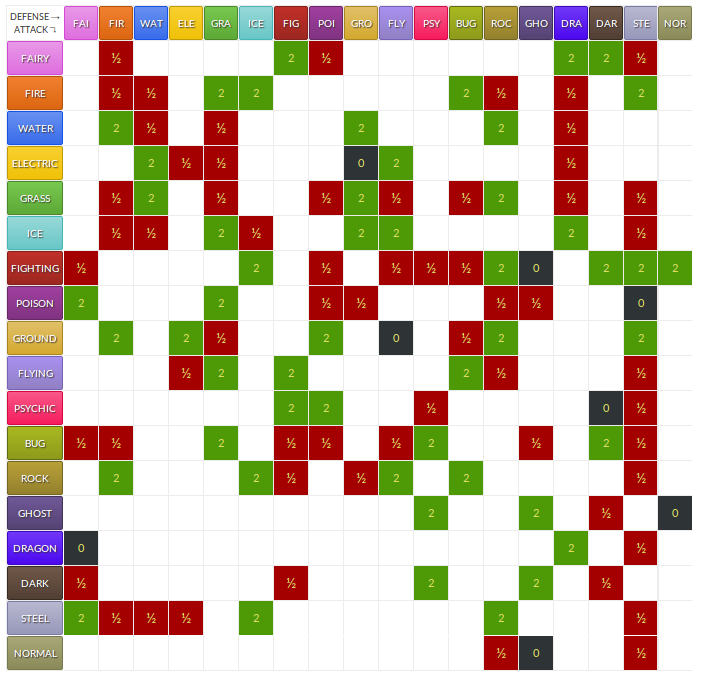
\includegraphics[width=\textwidth]{typeChart.png}
\end{center}
However, complications do often arise. Remember that every Pok\'emon species can have a minimum of 1, maximum of 2 types. Should a Pok\'emon have 2 types, then those types could cancel out each other's weaknesses with their resistances and vice versa. Another possible occurrence is that both types of the Pok\'emon of interest have the same weakness or resistance, resulting in the Pok\'emon being incredibly weak to or incredibly resistant against a certain type, respectively.\\\\
In other words, in competitive Pok\'emon battling, a trainer must try to form a team where the members
\begin{itemize}
	\item balance out each other's weaknesses with their resistances.
	\item have enough variety among themselves so that they can deal with as many different Pok\'emon and their associated types as possible.
\end{itemize}
The discussed Pok\'emon gameplay mechanics discussed above are the predominate factors that the SBPA algorithm will take into account. As stated previously, this algorithm is by no means perfect; it merely gives advice for the situation at hand. It ignores many gameplay mechanics that are far too complex to program into the algorithm in the allotted time for this project.

\section{The Mechanics Behind the Algorithm}
Now that the necessary background information has been established and documented, SBPA can be described in detail. SBPA is a computer algorithm written in Java. The author chose not to use Matlab or Maple as the main programming platform because Java is not only more convenient to share with other people, but also it deemed more useful to the author. This section will more describe the mathematical theory behind SBPA; software details will be ignored unless they have pertinence to the mathematics. The main code can be found in the appendix below.\\\\
SBPA is very input-driven; it relies heavily on the input of the user to run to completion. At the very beginning, the algorithm requires the Pok\'emon that the user wants to build a team around, the style of team the user wants to make (whether it be defensive, balanced, or aggressive), and which tiers the user wants to use. See Definition \ref{tierdef} for a reminder of what tiers are.\\\\
Every execution of the algorithm follows the same schedule.
\begin{enumerate}
	\item Gather the necessary information from the given situation. For one, this results in a (still quite large) list of Pok\'emon for the algorithm to run through.
	\item For every Pok\'emon in the list determined in the previously, apply a series of measures and give an overall score based on these measurements and the data gathered in the previous step.
	\item Sort the list in descending order based on the scores found in the previous step.
	\item Display the first $K$ results from the sorted list and wait until the user has chosen a Pok\'emon for his/her team based on the displayed suggestions or his/her own decision.
	\item Take the user's decision into account and repeat steps 1 through 4 until the user has a team of 6 Pok\'emon.
\end{enumerate}
In other words, SBPA takes into account the partial team that the user already has and suggests the best addition to that team based on a mathematics-based scoring system. However, there is no universal measure for deciding whether a Pok\'emon is a "good" or "bad" candidate for a team. Therefore, the scoring system is not based on an absolute scale, but rather a relative one, comparing Pok\'emon to each other to find the optimal solution. The scoring system takes 3 factors into account: a Pok\'emon's Base Stats, a Pok\'emon's Typing, and a Pok\'emon's Popularity Factor. These scoring factors build upon each other as depicted in the diagram below:
\begin{center}
	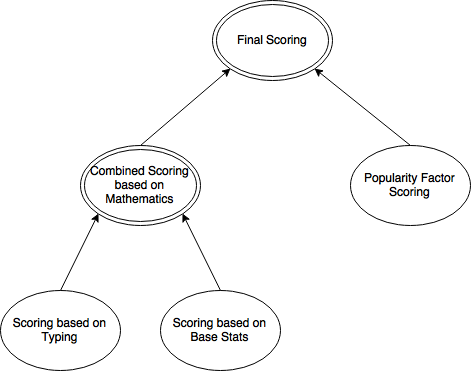
\includegraphics[width=0.7\textwidth]{ScoringDiagram.png}
\end{center}

\subsection{Scoring Based on Base Stats}\label{scoringBaseStats}
As discussed previously, the Base Stats of a Pok\'emon determine how well that Pok\'emon can fulfill certain roles in a team. Therefore, a logical approach to determining a score for a Pok\'emon is how well it fills the roles that the partial team of the user still needs to fill.\\\\
The algorithm does this by using the following equation:
\begin{equation}\label{statsScoreEqn}
	S(P,t)_{stats}=(\textbf{A}(t+P)-\textbf{A}(T))\cdot\textbf{M}_{stats}
\end{equation}
Here, $S(P,t)_{stats}$ stands for the score given to Pok\'emon $P$ relative to it's stats. The real vector $\textbf{A}(t+P)$ is the average Base Stats, in vector form, of the user's partial team $t$ with the addition of Pok\'emon $P$, whereby:
\begin{itemize}
	\item $A(t+P)_1$ is the average HP Base Stat of $P$ and all Pok\'emon in $t$
	\item $A(t+P)_2$ is the average Attack Base Stat of $P$ and all Pok\'emon in $t$
	\item $A(t+P)_3$ is the average Defense Base Stat of $P$ and all Pok\'emon in $t$
	\item $A(t+P)_4$ is the average Special Attack Base Stat of $P$ and all Pok\'emon in $t$
	\item $A(t+P)_5$ is the average Special Defense Base Stat of $P$ and all Pok\'emon in $t$
	\item $A(t+P)_6$ is the average Speed Base Stat of $P$ and all Pok\'emon in $t$
\end{itemize}
The vector $\textbf{A}(T)$ is constructed in a similar way; however it contains the average Base Stats of the Pok\'emon in the tier $T$ that the user is working with.\\\\
Vector $\textbf{M}_{stats}$ is the bias depending on the user's preference of team style. It may be possible that the user wants to construct a team that, for example, is more aggressive when compared to other teams. In that case, Attack, Special Attack, and Speed Base Stats are of more importance than HP, Defense, and Special Defense Stats. The bias vector $\textbf{M}_{stats}$ was therefore introduced in order to give more importance to Base Stats that matter more in the eyes of the user. The algorithm gives three options in team style: Defensive, Balanced, and Aggressive. The bias vector is then chosen as follows:
\begin{itemize}
	\item $\textbf{M}_{stats}=[\frac{3}{2},\frac{1}{2},\frac{3}{2},\frac{1}{2},\frac{3}{2},\frac{1}{2}]^T$ when the user builds a Defensive team;
	\item $\textbf{M}_{stats}=[\frac{1}{2},\frac{3}{2},\frac{1}{2},\frac{3}{2},\frac{1}{2},\frac{3}{2}]^T$ when the user builds an Aggressive team;
	\item $\textbf{M}_{stats}=[1,1,1,1,1,1]^T$ when the user builds a Balanced team;
\end{itemize}
The exact values of these vectors are based on author's choice to generate a noticeable difference between team styles. However, the values have been set in such a way that the sum of the elements in $\textbf{M}_{stats}$ is always equal to 6. This was done in order to preserve some semblance of equality and balance between the vectors.\\\\
In theory (and also of course in practice), this equation first scores Pok\'emon $P$ on the impact it would have when added to the partial team $t$, relative to the average Base Stats of tier $T$. This score is then combined with the previously discussed bias $\textbf{M}_{stats}$ into a dot product to result in a final scalar score. The dot product was chosen for two reasons. First of all, the dot product is a simplistic operation that is time-efficient and easy to understand. But more importantly, the dot product allows the scoring to take into account the influence of every Base Stat of $P$ and not just the largest or most important, as mere rudimentary examples. Thereby, SBPA can evaluate every Pok\'emon throughly based on it's Base Stats, yet still do this in an efficient manner.

\subsection{Scoring Based on Typing}
The SBPA algorithm also takes a Pok\'emon's typing into account in order to give it a score. Keeping track of a team's overall typing is important so that any glaring weaknesses or an excess investment in the resistance of a certain type can be avoided. Therefore, a Pok\'emon is scored based on the weaknesses, resistances, and immunities of the user's partial team.\\\\
In this case, the scoring follows the equation below:
\begin{equation}\label{typeScoreEqn}
	S(P,t)_{type}=(\textbf{T}(t+P)-\textbf{T}(t))\cdot\textbf{M}_{type}
\end{equation}
This equation is once again based on vectors and dot products. In this case, $S(P,t)_{type}$ is the score given to a Pok\'emon $P$ relative to it's typing.\\\\
Vector $\textbf{T(t)}$ is a integer vector that discribed how well partial team $t$ handles opposing Pok\'emon of a certain type. The vector needs to monitor how well $t$ interacts with all types; since there are 19 types (18 Pok\'emon types and 1 added NULL type for computational simplicity), $\textbf{T}(t)$ is 19 elements long. Element $T(t)_i$ is calculated in the following way:
\begin{itemize}
	\item $T(t)_i=T(t)_i-1$ if Pok\'emon $j$ of $t$ is weak to Type $i$
	\item $T(t)_i=T(t)_i+1$ if Pok\'emon $j$ of $t$ is resistant to Type $i$
	\item $T(t)_i=T(t)_i+2$ if Pok\'emon $j$ of $t$ is immune to Type $i$
\end{itemize}
The vector $\textbf{T}(t+P)$ is calculated much in the same way, except for the fact that it monitors how well $t$ would handle certain types if $P$ were to be added to it.\\\\
The bias vector $\textbf{M}_{type}$ is present in this equation to once again dictate what is more important and what is less important. At the moment, the types are dictated as being equivalently important for simplicity's sake, but a possible update to the program could be a bias vector $\textbf{M}_{type}$ based on the weaknesses and resistances of each type. More research in this field is necessary to discover how such a bias vector could be computed.\\\\
The equations \ref{statsScoreEqn} and \ref{typeScoreEqn} are structured in a similar way, and thus the mathematical theories behind both equations are almost identical. Just as in equation \ref{statsScoreEqn}, $S(P,t)$ is based on the typing benefits that Pok\'emon $P$ could add to partial team $t$. Once that has been computed, a dot product is taken with the bias vector $\textbf{M}_{type}$ in order to efficiently combine all elements of $(\textbf{T}(t+P)-\textbf{T}(t))$ and $\textbf{M}_{type}$ into a scalar value.

\subsection{Scoring Based on Popularity Factor}
As explained before, a Pok\'emon isn't defined merely by it's Base Stats and Typing. Unfortunately, most other characteristics are time-consuming to program and could not be included in the mathematics of the SBPA algorithm. However, a method was devised to still take these characteristics into account: the popularity factor $S(t,P)_{pop}$.\\\\
The popularity factor is based on the past experiences of other players. Since the Pok\'emon franchise is one of the most successful of all time, thousands of people battle every day (CITE?) in order to improve their skills and become the very best that they can be. With that many players, certain patterns start to evolve over time, centering around successful strategies. One could compare the world-wide group of Competitive Pok\'emon players as an immense, complicated computer program, its purpose being to seek out new battle strategies while preserving the those that result in a high success rate. The author found it foolish not to use the successful strategies that have been found thus far.\\\\
The popularity factor is not a mathematics-based construct; rather, it is based on collecting as many teams as possible for each tier and storing them efficiently to be used later. Therefore, the author constructed a matrix $\textbf{P}_T\in\mathbb{Z}^2$ for every tier $T$, wherein every Pok\'emon in that tier has its own separate column and and its own separate row. Therefore, the matrix for the tier that allows $k$ Pok\'emon to battle has $k$ columns and $k$ rows, resulting in $k^2$ different numbers.\\\\
At first, all the elements in these matrices are 0. Populating these matrices with useful data is done as follows.
Let's say the author finds a Pok\'emon team $t$, allowed by tier $T$, that he wishes to use as data for SPBA. He already has written a program to import any team he wishes in the algorithm. The program scans through $t$ and imports only the Pok\'emon species present in the team; all other characteristics are not included in order to decrease the algorithm's run time as much as possible. The program then finds the rows and columns in $\textbf{P}_T$ corresponding to each of the members of the team, and groups then into sets $R_t$ and $C_t$ respectively. The matrix $\textbf{P}_T$ is then updated as follows:
\begin{equation*}
	\textbf{P}_{T,r,c}=\textbf{P}_{T,r,c}+1\text{, }r\in R_t\text{ and }c\in C_t
\end{equation*}
In this way, $\textbf{P}_T$ is build to register patterns between Pok\'emon in the same team. The higher the element of $\textbf{P}_T$, the more people use the corresponding two Pok\'emon in a team, and thus the more likely that the two corresponding Pok\'emon work well together. What is more, this method does not depend on Pok\'emon Base Stats or Typing, resulting in a simple method capable of finding effective Pok\'emon team combinations that would otherwise go unnoticed in the analysis of Base Stats and Typing.\\\\
Understanding all this, the popularity factor is simple to express for a partial team $t$ allowed in tier $T$ and possible new team member $P$:
\begin{equation}\label{popScoreEqn}
	S(t,P)_{pop}=\sum_{s\in t}\textbf{P}_{T,s,P}
\end{equation}
In other words, $S(t,P)_{pop}$ is simply a measure to see how many times Pok\'emon $P$ and a member of partial team $t$ have been in a team in the past.

\subsection{Combining Scoring factors}
Combining equations \ref{statsScoreEqn}, \ref{typeScoreEqn}, and \ref{popScoreEqn} takes some thought. As stated previously, there is no universal measure for deciding whether Pok\'emon $P$ is a "good" or "bad" candidate for partial team $t$. Rather, the final score given to $P$ should be relative: how well $P$ scores in comparison to all the other candidates.\\\\
The author decided to combine the scoring systems in such a way to meet the following criteria:
\begin{enumerate}
	\item Results for equation \ref{typeScoreEqn} should be about 1.4 times as important as results from equation \ref{statsScoreEqn}. This observation comes from Jenty Heijstek, a competitive trainer who (CITE). Furthermore, Equations \ref{statsScoreEqn} and \ref{typeScoreEqn} should be combined into one scoring system based on mathematics alone, with Equation \ref{popScoreEqn} added later. In this way, a Pok\'emon can be analyzed not only mathematically, but also based on popularity, resulting in a simple, but varied methodology of analysis.
	\item Importance of equation \ref{popScoreEqn} should decrease as more Pok\'emon add added to the team, while at the same time, the importance of the scoring sytem based on equations \ref{statsScoreEqn} and \ref{typeScoreEqn} should increase. As a team nears completion, all imperfections and glaring flaws need to be compensated for, which is much more easily done when analyzing a Pok\'emon's Base Stats and Typing than a Pok\'emon's popularity. 
\end{enumerate}

\subsubsection{Criteria 1}
The first criteria can easily be met by performing the following linear transformations on $S(t,P)_{stats}$ and $S(t,P)_{type}$:
\begin{eqnarray*}
	S'(t,P)_{stats}=(S(t,P)_{stats}-\min_P(S(t,P)_{stats}))*\cfrac{10}{\max_P(S(t,P)_{stats})-\min_P(S(t,P)_{stats})}\\
	S'(t,P)_{type}=1.4*(S(t,P)_{type}-\min_P(S(t,P)_{type}))*\cfrac{10}{\max_P(S(t,P)_{type})-\min_P(S(t,P)_{type})}
\end{eqnarray*}
Through this transformation, both $S(t,P)_{stats}$ and $S(t,P)_{type}$ are changed to always have a range equal to the interval [0,10], thereby removing any bias that could result from the two scoring systems having different ranges. Unfortunately, these transformations needs to be performed every iteration of the algorithm since $\max_P(S(t,P)_{stats})$, $\min_P(S(t,P)_{stats})$, $\max_P(S(t,P)_{type})$, and $\min_P(S(t,P)_{type})$ ae different values for every iteration. But a computer can easily perform a linear transformation, so thankfully not much time is lost during this step.\\\\
Now define a new scoring system $S(t,P)_{math}$ that can be expressed as follows:
\begin{equation*}
	S(t,P)_{math}=S'(t,P)_{stats}+1.4*S'(t,P)_{type}
\end{equation*}
In this way, $S'(t,P)_{type}$ has a 1.4 times more influence than $S'(t,P)_{stats}$. 
Now define the final score as follows:
\begin{equation*}
	S(t,P)_{final}=f(S(t,P)_{math},S(t,P)_{pop})
\end{equation*}
The function $f(S(t,P)_{math},S(t,P)_{pop})$ must be defined with the help of Criteria 2.

\subsubsection{Criteria 2}
Meeting Criteria 2 can be done by defining $S(t,P)_{final}$ as follows:
\begin{equation*}
	S(t,P)_{final}=c_1(t)*S(t,P)_{math}+c_2(t)*S'(t,P)_{pop}
\end{equation*}
In this case, $S(t,P)_{final}$ is defined as the weighted sum of $S(t,P)_{math}$ and $S'(t,P)_{pop}$, whereby $S'(t,P)_{pop}$ is a linear transformation much like the ones performed to $S(t,P)_{stats}$ and $S(t,P)_{type}$ to meet Criteria 1. In this case, author wants to avoid any unintended bias from the possibility that the functions $S(t,P)_{math}$ and $S(t,P)_{pop}$ have differing ranges. Since $S(t,P)_{math}$ is defined on the interval [0,20], $S'(t,P)_{pop}$ can be defined as follows:
\begin{equation*}
	S'(t,P)_{pop}=(S(t,P)_{pop}-\min_P(S(t,P)_{pop}))*\cfrac{20}{\max_P(S(t,P)_{pop})-\min_P(S(t,P)_{pop})}
\end{equation*}
The weights $c_1(t)$ and $c_2(t)$ differ as $t$ grows. They are not so much dependent on $t$ itself, but more on $|t|$, or how many members $t$ already contains. Also, since the author wants the importance of $S(t,P)_{math}$ to increase as the importance of $S'(t,P)_{pop}$ decrease, and vice versa, $c_2(t)$ was chosen to be equal to $1-c_1(t)$, assuming that $c_1(t)\text{, }c_2(t)\in[0,1]\in\mathbb{R}$.\\\\
Since $|t|\in [0,6]\in\mathbb{Z}$, $c_1(t)$ and $c_2(t)$ can only assume a limited amount of values. Taking into account that SBPA must start with a partial team that atleast has 1 member, and that the algorithm doesn't need to analyze a team of 6 since then it is complete, the author decided to define the values of $c_1(t)$ as follows:
\begin{center}
	\begin{tabular}{c||c|c|c|c|c}
		$|t|$&1&2&3&4&5\\
		\hline
		$c_1(t)$&1/3&1/2&2/3&4/5&9/10
	\end{tabular}
\end{center}
Besides the author's intuition after having participated in hundreds of Pok\'emon battles, several factors went into deciding these constants
\begin{itemize}
	\item When $|t|=1$, a trainer usually looks for Pok\'emon that strengthen a certain strategy he/she has in mind. Although Typing and Base Stats are of importance, using the popularity factor is a much better method for finding interesting and effective Pok\'emon partners.
	\item When $|t|=2$, $t$ needs to start compensating for unbalanced Typings and Base Stats while still paying attention to what other trainers have made over the years. Roughly at this point, the importance of $S(t,P)_{math}$ and $S'(t,P)_{pop}$ are about equal.
	\item When $|t|>2$, the importance of $S(t,P)_{math}$ grows asymptotically to 1, while the importance of $S(t,P)_{pop}$ decreases at the same rate to 0. Less and less does $t$ need to take heed of what other trainers have done in the past; what the team needs more and more is to become whole while compensating for as many weaknesses and flaws as possible.
\end{itemize}
Other competitive Pok\'emon trainers agreed with these choices for constants as well, including (JENTY)\\\\
All in all, the scoring system for analyzing a Pok\'emon $P$ for partial team $t$ is done as follows:
\begin{eqnarray*}
	S(t,P)_{final}=c_1(t)*(S'(t,P)_{stats}+1.4*S'(t,P)_{type})+(1-c_1(t))*S'(t,P)_{pop}\\
	S'(t,P)_{stats}=(S(t,P)_{stats}-\min_P(S(t,P)_{stats}))*\cfrac{10}{\max_P(S(t,P)_{stats})-\min_P(S(t,P)_{stats})}\\
	S'(t,P)_{type}=(S(t,P)_{type}-\min_P(S(t,P)_{type}))*\cfrac{10}{\max_P(S(t,P)_{type})-\min_P(S(t,P)_{type})}\\
	S'(t,P)_{pop}=(S(t,P)_{pop}-\min_P(S(t,P)_{pop}))*\cfrac{20}{\max_P(S(t,P)_{pop})-\min_P(S(t,P)_{pop})}
\end{eqnarray*}

\section{Run-Time Analysis}
The SBPA algorithm is a much more time-efficient method of giving suggestions for Pok\'emon team building than, say, brute force calculations. Brute forcing the problem has its merits, of course, the most predominate being able to specifically calculate the absolute best team; however doing such a calculation would cost so much time and data that this methodology loses it's validity rather quickly. But the question still remains: how fast is SPBA?\\\\
To answer this question, the author performed a multitude of test runs and recorded the run time of each test. The tests were designed as follows:
\begin{enumerate}
	\item Choose a team style (Defensive, Balanced, or Aggressive. See Section \ref{scoringBaseStats}). Do this merely for consistency's sake; the choice of team style should not affect the elapsed runtime of the algorithm.  
	\item Choose a tier $T$
	\item Choose a team of 6 Pok\'emon at random and input the team one Pok\'emon at a time, keeping track of the elapsed runtime for each iteration
	\item Repeat the third step 10 times.
	\item Repeat steps 1-5 for each tier not equal to $T$
\end{enumerate}
For his experimentation, the author used the Defensive team style. The following 7 charts shows the resulting elapsed runtimes per iteration for all the test runs in milliseconds:
\begin{center}
	\begin{tabular}{c||c|c|c|c|c|c|c|c|c|c||c}
		AG&Test 1&Test 2&Test 3&Test 4&Test 5&Test 6&Test 7&Test 8&Test 9&Test 10&Averages\\
		\hline\hline
		It. 1&764&565&613&648&571&577&575&640&621&663&623.7\\
		It. 2&594&578&659&650&637&644&633&604&674&731&640.7\\
		It. 3&312&284&288&321&274&297&306&293&319&329&302.3\\
		It. 4&250&216&273&294&298&293&255&273&251&302&270.5\\
		It. 5&339&237&311&370&315&307&310&341&269&315&311.4\\
	\end{tabular}
\end{center}
\begin{center}
	\begin{tabular}{c||c|c|c|c|c|c|c|c|c|c||c}
		Ubers&Test 1&Test 2&Test 3&Test 4&Test 5&Test 6&Test 7&Test 8&Test 9&Test 10&Averages\\
		\hline\hline
		It. 1&686&617&631&621&632&600&634&701&633&659&641.4\\
		It. 2&667&655&624&610&650&659&633&577&580&609&626.4\\
		It. 3&298&295&275&296&297&308&273&281&315&309&294.7\\
		It. 4&286&291&244&262&281&252&273&256&265&255&266.5\\
		It. 5&283&303&219&278&301&292&259&317&281&341&287.4\\
	\end{tabular}
\end{center}
\begin{center}
	\begin{tabular}{c||c|c|c|c|c|c|c|c|c|c||c}
		BS&Test 1&Test 2&Test 3&Test 4&Test 5&Test 6&Test 7&Test 8&Test 9&Test 10&Averages\\
		\hline\hline
		It. 1&723&624&554&603&603&625&642&582&589&589&613.4\\
		It. 2&309&414&329&308&289&292&341&288&345&260&317.4\\
		It. 3&299&668&593&569&552&573&588&586&581&525&553.4\\
		It. 4&228&253&230&206&256&206&257&277&286&304&250.3\\
		It. 5&314&320&299&264&284&252&282&300&299&299&291.3\\
	\end{tabular}
\end{center}
\begin{center}
	\begin{tabular}{c||c|c|c|c|c|c|c|c|c|c||c}
		OU&Test 1&Test 2&Test 3&Test 4&Test 5&Test 6&Test 7&Test 8&Test 9&Test 10&Averages\\
		\hline\hline
		It. 1&605&597&587&608&620&593&610&633&598&538&598.9\\
		It. 2&403&289&306&369&365&293&328&295&281&355&328.4\\
		It. 3&648&627&526&656&682&550&620&618&589&598&611.4\\
		It. 4&279&227&184&329&236&204&213&228&251&266&241.7\\
		It. 5&275&271&271&286&258&302&278&259&288&287&277.5\\
	\end{tabular}
\end{center}
\begin{center}
	\begin{tabular}{c||c|c|c|c|c|c|c|c|c|c||c}
		UU&Test 1&Test 2&Test 3&Test 4&Test 5&Test 6&Test 7&Test 8&Test 9&Test 10&Averages\\
		\hline\hline
		It. 1&523&536&546&537&554&561&515&523&539&532&536.6\\
		It. 2&327&274&304&278&364&369&331&252&375&254&312.8\\
		It. 3&324&303&281&232&302&307&269&242&337&294&289.1\\
		It. 4&278&210&304&209&213&285&211&215&299&253&247.7\\
		It. 5&225&211&221&198&232&255&212&222&226&195&219.7\\
	\end{tabular}
\end{center}
\begin{center}
	\begin{tabular}{c||c|c|c|c|c|c|c|c|c|c||c}
		RU&Test 1&Test 2&Test 3&Test 4&Test 5&Test 6&Test 7&Test 8&Test 9&Test 10&Averages\\
		\hline\hline
		It. 1&504&466&429&449&487&464&485&431&470&424&460.9\\
		It. 2&245&279&294&316&311&296&300&293&278&304&291.6\\
		It. 3&412&411&265&272&280&242&257&303&286&287&301.5\\
		It. 4&168&168&185&188&216&167&198&214&180&187&187.1\\
		It. 5&208&200&250&224&253&221&179&231&191&235&219.2\\
	\end{tabular}
\end{center}
\begin{center}
	\begin{tabular}{c||c|c|c|c|c|c|c|c|c|c||c}
		NU&Test 1&Test 2&Test 3&Test 4&Test 5&Test 6&Test 7&Test 8&Test 9&Test 10&Averages\\
		\hline\hline
		It. 1&442&389&401&410&414&391&407&430&389&411&408.4\\
		It. 2&325&224&241&261&241&217&221&227&255&288&250.0\\
		It. 3&287&244&253&243&233&283&316&243&272&279&265.3\\
		It. 4&215&188&237&200&187&158&235&179&168&190&195.7\\
		It. 5&167&157&175&143&147&139&166&156&147&156&155.3\\
	\end{tabular}
\end{center}
The following graph visualizes the averages:
\begin{center}
	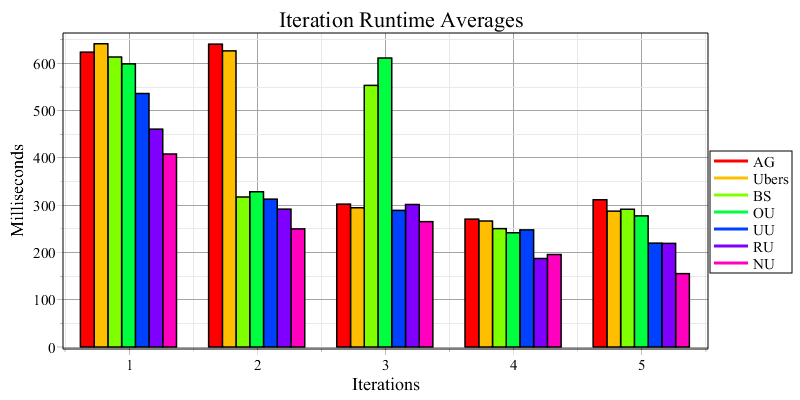
\includegraphics[width=\textwidth]{RuntimeAverages.png}
\end{center}
The data indicates some note-worth phenomena:
\begin{enumerate}
	\item In general, the more Pok\'emon are allowed by a tier, the longer it takes for SPBA to search for an optimal partner. This was rather expected, since less data to process equates to less time to process. What is of interest is that there seems to be a linear correlation between the amount of Pok\'emon that a tier allows and the time required for SBPA to complete an iteration, as shown between the graph shown above and in Section \ref{TierAmountGraph}. Whether this is a true linear correlation is hard to say: the possibility exists that there isn't enough data for the algorithm to start exhibiting non-linear characteristics. Only through the making of tiers can this hypothesis be tested.
	\item In general and per tier, every iteration in the SBPA algorithm seems to take less time. This occurrence is again to be expected for much the same reason as phenomena 1: every iteration processes less and less data by ignoring all Pok\'emon (and forms thereof) that have already been selected for the user's team.
	\item At the second iteration for tiers BS (BattleSpot Singles) and OU (Over Used), the SPBA algorithm requires around 325 milliseconds to run to completion. However, the iteration takes almost twice as long. This phenomena is odd, since it does not occur for any other tier and defies all logic. Perhaps this occurrence results from faulting programming somewhere in the algorithm, but more research is needed to discover its origin.
	\item At the second iteration, the algorithm requires around 300 milliseconds to run to completion all but two tiers. However, for the AG (Anything Goes) and Ubers tiers, SPBA still requires around 640 milliseconds. Both tiers include the same Pok\'emon species, save for one form, which explains why the graphs for these two tiers are so similar. However, it does not explain why the algorithm requires much less time to complete iteration 2 for all other tiers. More research is required to investigate this matter.
\end{enumerate}

\section{Conclusion}
The SBPA algorithm is an algorithm that gives advice on how to build a competitive Pok\'emon team in order for trainers to get a start on a team which they can later on perfect. It uses simple mathematics to analyze Pok\'emon species on an individual level and determine the best potential team members based on Base Stats, Typing, and the popularity factor.\\\\
SBPA focuses on time efficiency. Through experimentation and algorithm runtime analysis, it has been shown that the algorithm can complete any iteration in less than a second, which is astronomically more time efficient than analyzing every possible combination of Pok\'emon species in order to find an optimum. All be SBPA less accurate in determining the absolute optimum, the efficiency is compensation enough.\\\\
The author does plan to continue developing SBPA into an even more accurate, streamline program that hopefully one day will be available for all trainers alike.

\newpage
\section{Acknowledgments and Bibliography}
http://www.pokemon.com/us/about-pokemon/\\
Reference to "Pocket monsters"\\
Jenty Heijstek 10/6/2016\\
fluffy photo\\
fluffy file\\
type chart

\section{Appendix}

\end{document}